\chapter{Implementation}




\section{Compression}
\label{section:impl_compression}

To compress the BTF data we used Java programming language. In our case, the main problem of PCA lies in implementation of singular value decomposition (SVD).
To solve this problem, we used a fast linear library \emph{jblas} \cite{jblas} developed by Mikio Braun. The \emph{jblas} library is gaining popularity in scientific computing.
This library is one of the most fastest library for the Java programming that can solve various linear algebra problems. 

Compressed data has to be sent to a shader. The best way to send matrices to a shader, is to send them as textures. 
So, after we perform SVD, we save our resulted matrices $U$, $\Sigma$, $V$ as textures.  Matrices $U$ and $V$ are in range $[-1;1]$, so we map the data into image domain $[0;1]$.
We store each component of matrix $U$ separately as PNG images. We store each component separately as we would need to stream the data.
Consider an example shown in Figure \ref{fig:compr}, which shows first components of some materials.
Matrices $\Sigma$ and $V$ are stored together in one texture as they are small enough. Note that the values of matrix $\Sigma$ are not in range $[-1;1]$, but we are still able to map them and store in the texture.
We will not go in details here, as it is a trivial task.

Also, one practical consideration when using \emph{jblas} is to scale the data for better reconstructing quality in the shader. We found out that tenths of values of $U$ and $V$ matrices are zeros.
So, basically we can scale the data by multiplying it with $10$ and at the same time matrix $\Sigma$ by $0.1$. This way the reconstruced resulted will the same. But, with scaling we improves precision of the data when we map it.




\begin{figure}[h]
 \centering
 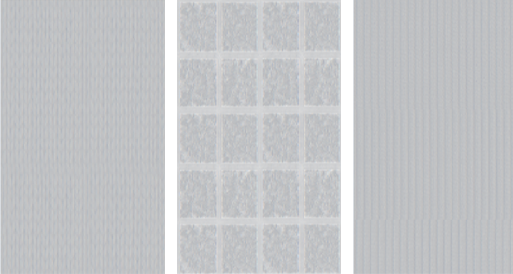
\includegraphics[width=0.7\textwidth]{figures/compr}
 \caption[Example of Principal Components] {
 	{\bf Example of Principal Components }
	
	\textbf{From left to right}: wool, impalla, corduroy. 
 }
 \label{fig:compr}
\end{figure}


\section{Rendering}
\label{section:impl_rendering}


The aim of this thesis was to implement efficient BTF-shader for XML3D \cite{xml3d}. XML3D platform was implemented to deploy 3D graphics in web browsers. This technology is based on WebGL and JavaScript.
We also use Xflow \cite{xflow} to combine principal component textures in one texture, which further is needed for BTF-shader. The shader is written in OpenGL Shading Language (GLSL). 
The rendering process of the shader is depicted in figure \ref{fig:shader}.

The compressed BTF data is stored in two textures. One texture $L$ stores principal components, the other $R$ stores PCA weights, which determine how the components have to be summed up.
The other inputs are texture coordinates, eye and light positions. Eye and light positions are transformed to spherical coordinates.
 Then, we lookup the three closest views from the measured BTF data, which are will be needed for interpolation purpose.
 This lookup process is fairly simple as we have a static array in the shader, which stores sample intervals of the measured BTF data.

 




\begin{figure}[h]
 \centering
 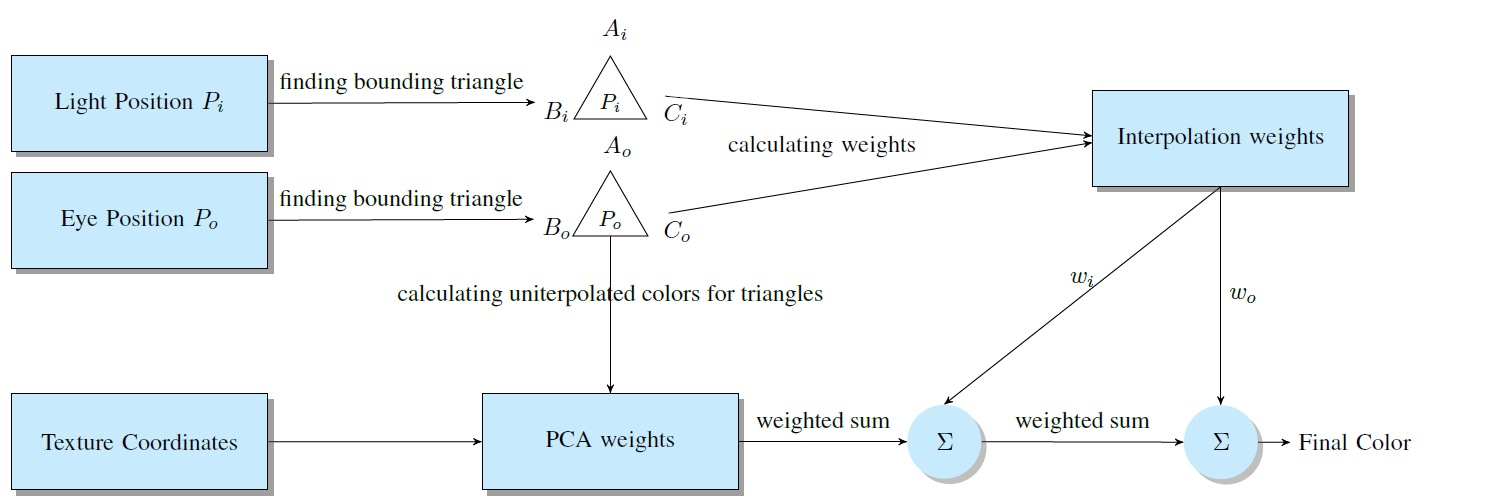
\includegraphics[width=1.0\textwidth]{figures/shader}
 \caption[Shader Design] {
 	{\bf Shader Design }

 }
 \label{fig:shader}
\end{figure}


\section{Streaming}
\label{section:impl_streaming}


Xflow is a part of XML3D implementation, which allows to process the data on flow, i.e. in runtime.
At start, on a client side we create array \emph{texData} of RGB colors, which further will be fulfilled with newly arrived principal components. 
As it was described in chapter \ref{section:streaming}, we stream principal components one by one. Each component $C_{i}$ arrives as a PNG image. 
Then, on a client side we read PNG image using PNG decoder written in JavaScript by Arian Stolwijk \cite{pngreader}.
PNG images are decoded to pure array of RGB colors. This new data of component $C_{i}$ is then placed to its place in \emph{texData}  array. Finally, using Xflow we create from \emph{texData}  array a texture with which we update our BTF-shader.



\label{chapter:implementation}
